\documentclass[12pt]{report}
\usepackage[utf8]{inputenc}
\usepackage{graphicx}
\usepackage{amsmath}

\title{Information theory and data mining}
\author{Ivan Riolo }
\date{February 2021}

\begin{document}
\maketitle
\tableofcontents


\chapter{Assignment 1}
\section{Test COVID 19}
The first request for the assignment foresees to locally clone two git repositories concerning the statistics on the national and global data of covid 19:
\begin{itemize}
\item https://github.com/pcm-dpc/COVID-19.git
\item https://github.com/CSSEGISandData/COVID-19
\end{itemize}
This request is solved using the pygit2 package. By adding an initial check the repositories are downloaded only if they do not yet exist in the local directory, otherwise they are simply updated by running the git  pull command.
\begin{figure}[h!]
    \centering
    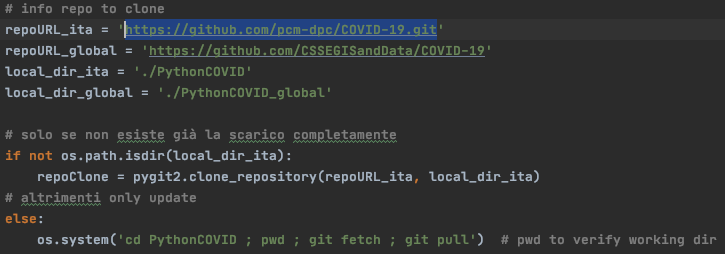
\includegraphics[width=14cm]{Pictures/covid1.png}
    \caption{pygit solution}
\end{figure}
The last request is to produce a plot of all the 'new positives' as a function of the days starting from the earliest available date up to the latest.
First is necessary to access the files in question (csv) and read their contents, to do this is possible to use the Pandas library. Through the take() method it is possible to copy the columns of interest in a local vector, in this case the 'new positive' column is extracted from the target file.
To create a graph that shows the trend of the extracted data it is possible to use the Numpy library, by means of the linspace() method the domain is created, it generates a one-dimensional vector of equally spaced intervals.
Then with the method plot() the graph is created providing the vector x of the domain and the vector y of the values, finally through the show() method the following result is shown.
\begin{figure}[h!]
    \centering
    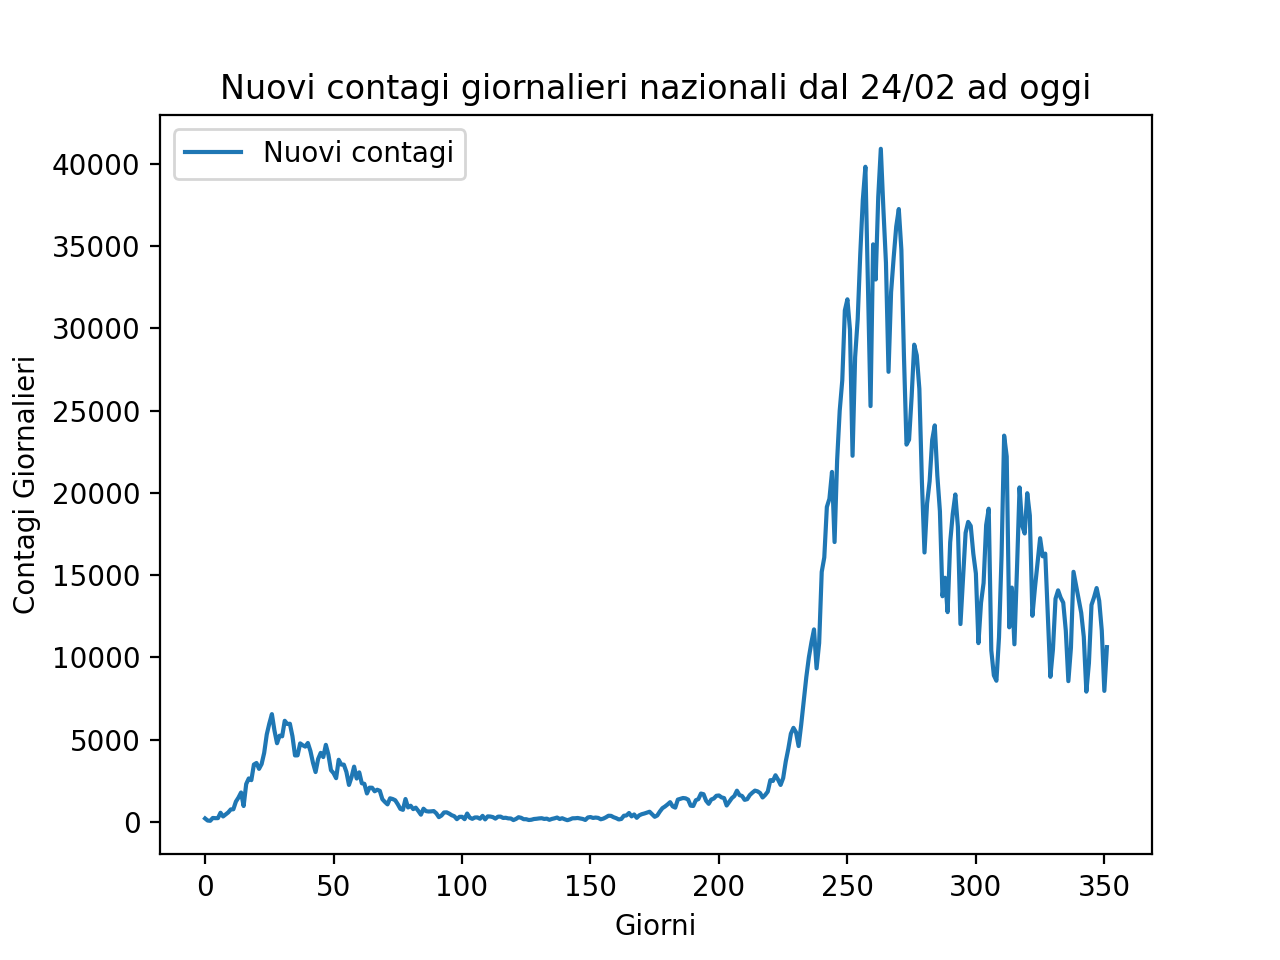
\includegraphics[width=14cm]{Pictures/covid2.png}
    \caption{daily national positives}
\end{figure}

It is possible to represent the same graph using global data concerning all the states of the world. In this case the data is saved differently, we have a table in which each row is a state and each column is a day. Therefore, to obtain the number of total daily infections it is necessary to add up each column. It's possible to use sum() method of pandas and the result is shown in the next figure.

\begin{figure}[h!]
    \centering
    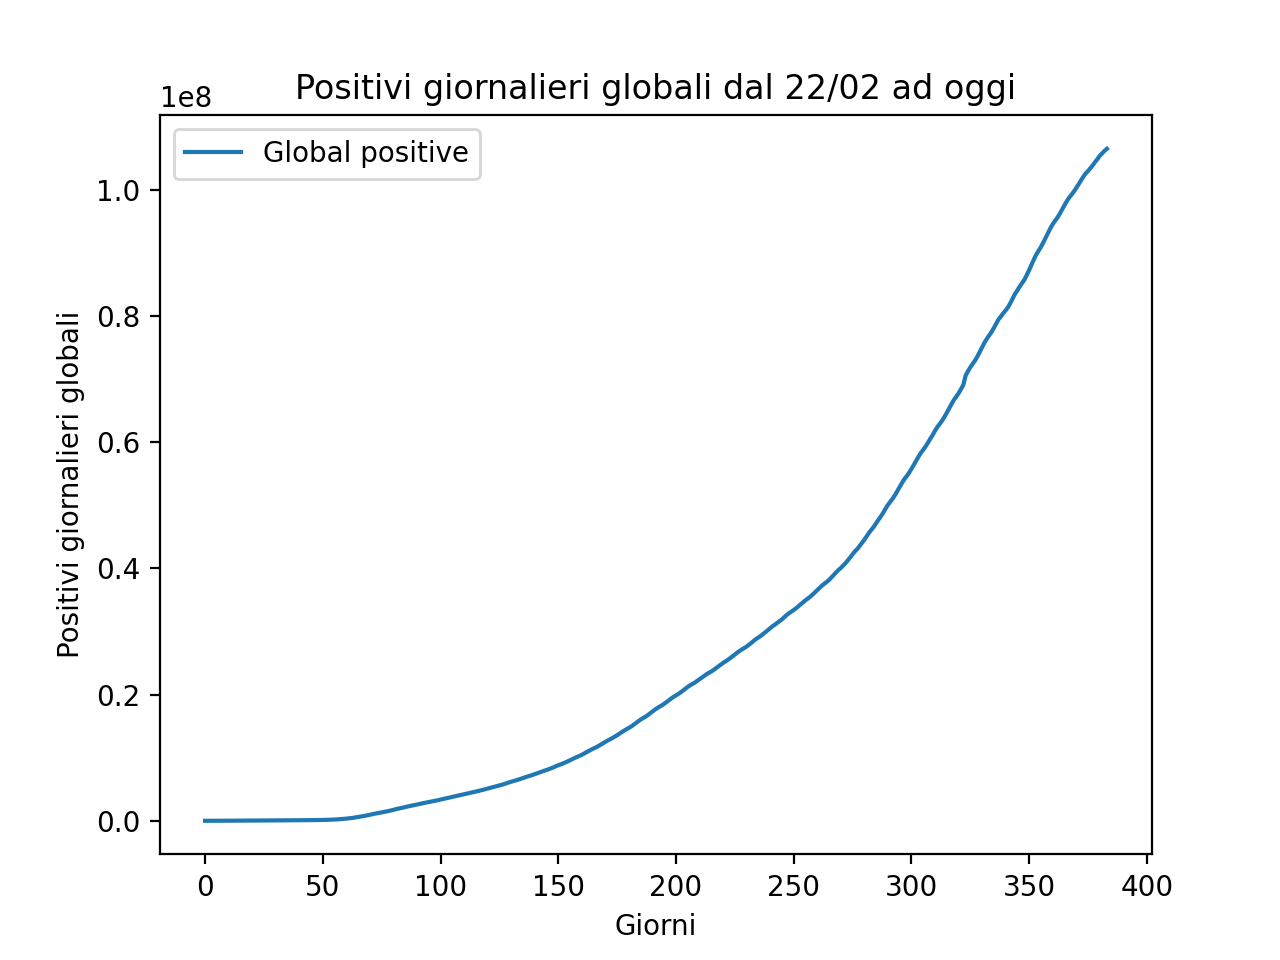
\includegraphics[width=14cm]{Pictures/covid4.png}
    \caption{daily global positives}
\end{figure}


\chapter{Assignment 2}
\section{Entropy function}
The first requirement is to implement the entropy function, having as an input parameter the probability mass of a discrete random variable. Consequently the input parameter is a vector of the type [p1, p2, ... pN]. To implement the summation that makes up the body of the entropy function is possibile to use a for loop as follows.

\begin{figure}[h!]
    \centering
    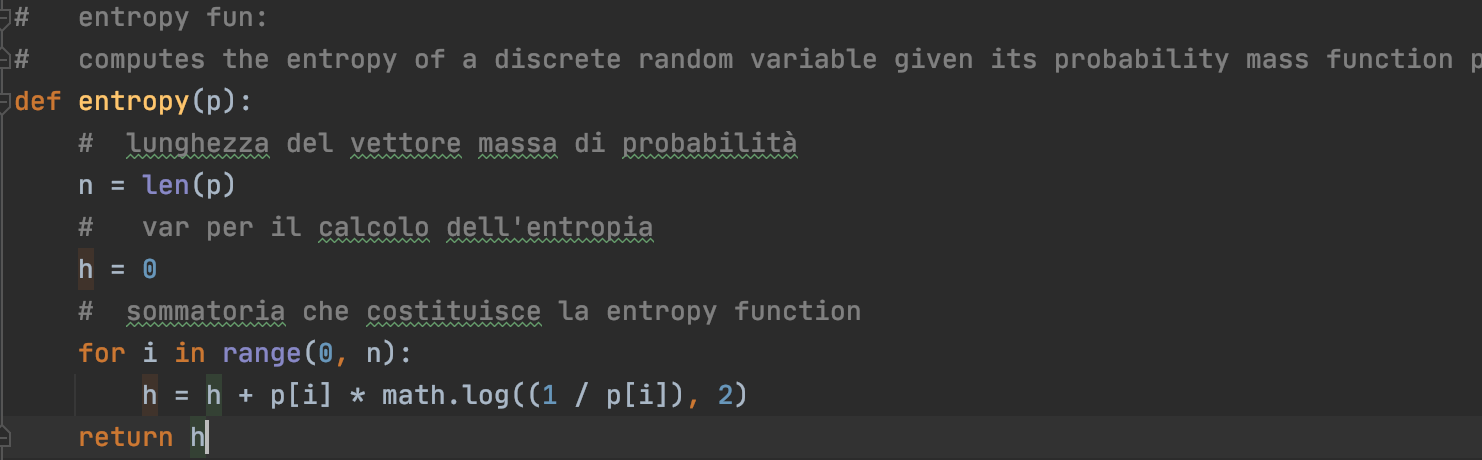
\includegraphics[width=14cm]{Pictures/entropy.png}
    \caption{Entropy function}
\end{figure}

It's important to note that is possible to use any base log value to measure information, in this case it's used base 2 according with bit definition.
The return of this function is a vector of the same length of the input probability mass function.
Recalling that entropy measures the amount of average information contained in each realization of the random variable is a very useful function during operations on large amounts of data. The next request is to use the newly created function by calculating the entropy of a binary r.v. as a function of $p0$ (the probability that event 1 will occur while $1 - p0$ is the probability of event $0$). In order to show the entropy trend of a generic binary random variable as a function of $p0$ through a plot, it is necessary to choose a very small sampling step, $0.0001$ in the example. In this way, the evenly spaced intervals on the x axis of the graph will be $1000$. It is possible to create the domain vector using the linspace() method and for each value inside it the entropy is calculated by using the precedent entropy function through a for loop. The result is the follow.

\begin{figure}[h!]
    \centering
    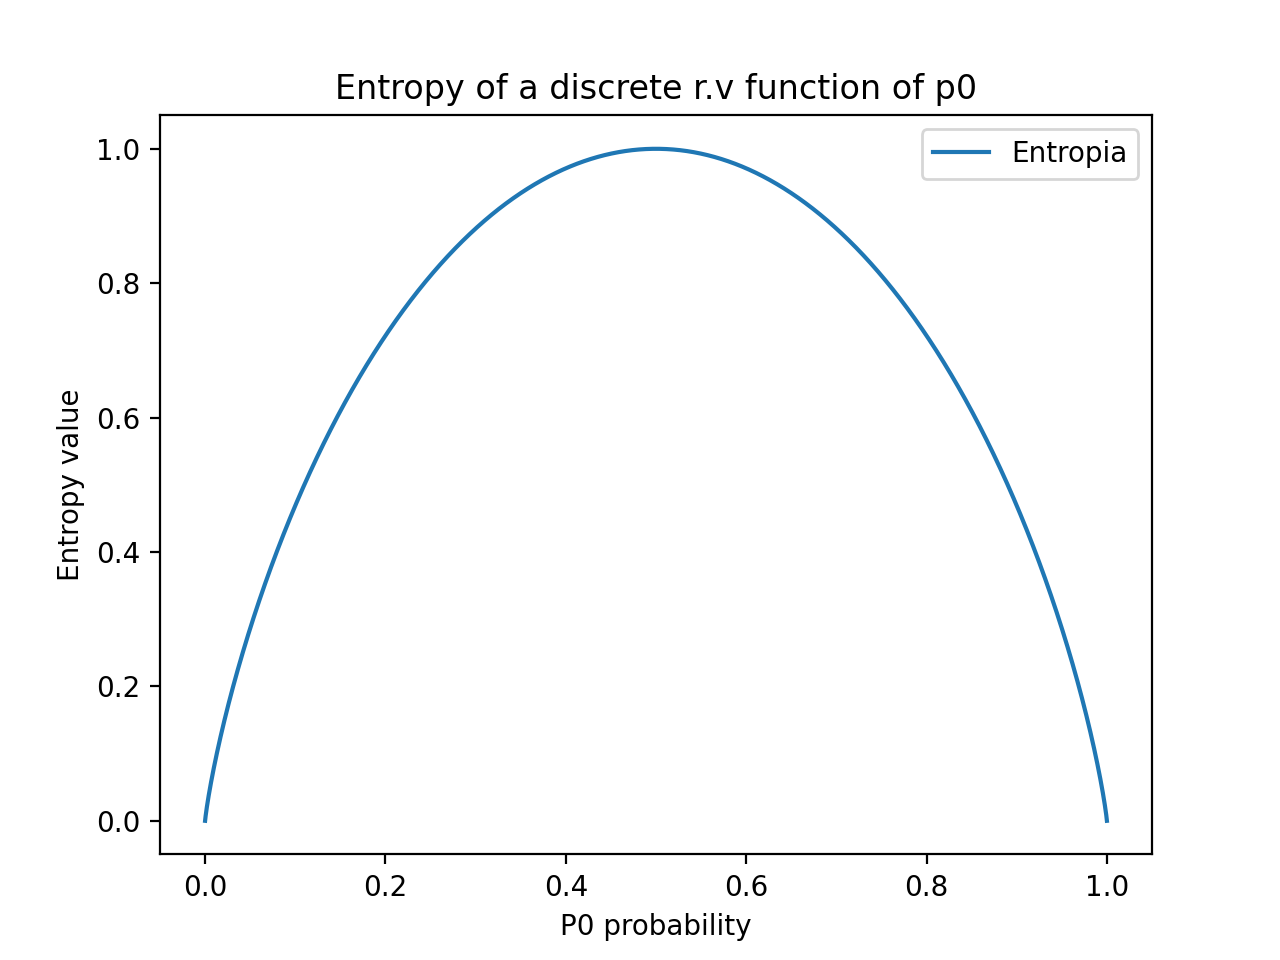
\includegraphics[width=14cm]{Pictures/entropy-test.png}
    \caption{Entropy of binary r.v}
\end{figure}

As it is possible to observe the maximum value of the entropy is obtained only when the discrete binary random variable is equiprobable, that is with probability 0.5 the favorable event occurs and with probability 0.5 the opposite event. This shows that entropy is also a measure of the degree of uncertainty placed in an event. In fact, when the uncertainty is maximum (the events are equiprobable) the information that contains is maximum.

\section{Joint entropy}
The joint entropy is defined in the same way as entropy but in this case is a measure for the joint probability and consequently a double summation is needed, as before, can be implemented through two for loops. Joint probability can be implemented through a 2D numpy array. Having the joint probability as input parameter, return as output the joint entropy.
\begin{figure}[h!]
    \centering
    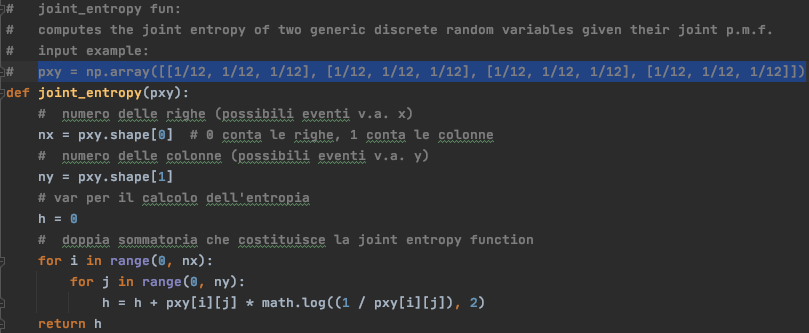
\includegraphics[width=14cm]{Pictures/joint entropy.png}
    \caption{Joint entropy function}
\end{figure}

It is important to recall that if the two random variables are independent then the joint probability can be expressed as the product of the marginal probabilities. It follows that the joint entropy in case of independents r.v can assume at most the sum value of the single entropies of x and y.

\section{Conditional entropy}
Considering the conditional probabilities of two events X and Y, the conditional entropy can measure the uncertainty on a value X after having observed value Y. It's defined the same as joint entropy but in this case in the argument of log there is the conditional probability of X observed Y. Considering that the function accept in input the joint probability of x and y and the marginals probabilities, it's possible to express the conditional prob. as the joint probability divided by marginal prob. of conditioning event by invert the chain rule:  $p(x,y) = p(x|y) * p(y) $. The result is the follow.
\begin{figure}[h!]
    \centering
    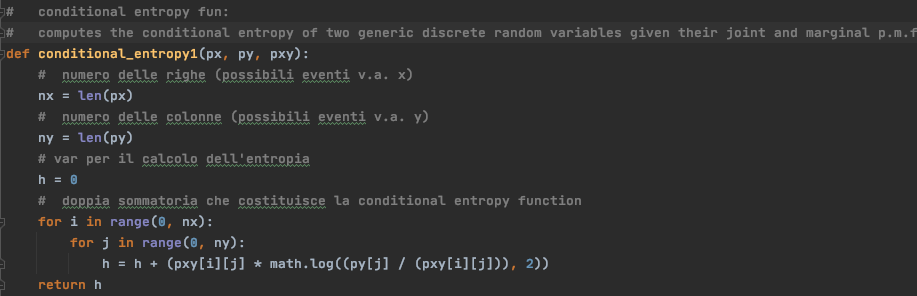
\includegraphics[width=14cm]{Pictures/Conditional entropy.png}
    \caption{Conditional entropy function}
\end{figure}

The max value that conditional entropy can assume is the marginal entropy of X in case X and Y are independent and the min value is 0 in case Y is function of X.

\section{Mutual information}
The mutual information is a measure of how similar are the joint probability $p(x,y)$ and the product of marginal probabilities $p(x) * p(y) $. In this case the max value is achieved when X and Y r.v. are dependent while low value of mutual information are produced when the r.v. are nearly independent.

\begin{figure}[h!]
    \centering
    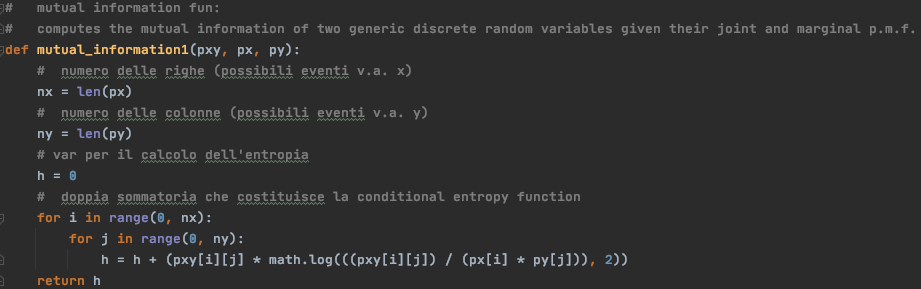
\includegraphics[width=14cm]{Pictures/Mutual information.png}
    \caption{Mutual information function}
\end{figure}

\section{Normalized functions}
Considering that in the bivariate case is possible to classify the information measures in two different groups:
\begin{itemize}
\item Similarity measures:
    \begin{itemize}
        \item Like mutual information are measures that increase with addiction between 2 r.v. 
    \end{itemize}
\item Dissimilarity measures:
\begin{itemize}
        \item Like conditional entropy are measures that increase with independence of 2 r.v.
    \end{itemize}
\end{itemize}
Consequently, normalization process is very useful when is needed to change the limits of the original domain measurements, as in the case of conditional entropy its domain is: $ 0<H(X|Y)<H(X)$ . Normalization of conditional entropy is achieved by divide it for entropy, follow that domain change in [0,1] instead of $ 0<H(X|Y)<H(X)$. The joint entropy is normalized by dividing it for the sum of marginal entropy $H(Y) + H(X)$, while the mutual information is normalized by dividing it for joint information $H(Y,X)$. The result recalling the precedent functions are the follow.

\begin{figure}[h!]
    \centering
    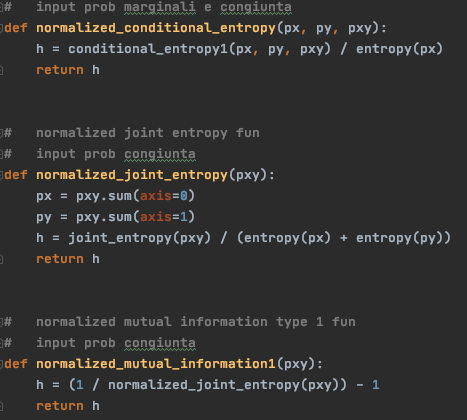
\includegraphics[width=10cm]{Pictures/Normalized fun.png}
    \caption{Normalized information function}
\end{figure}


\chapter{Assignment 3}
\section{Pmf estimator}
The first requirement is to calculate the difference between the entropy of a discrete random variable given its prior probability mass function, and the entropy of the same discrete random variable but by estimating its probability mass function starting from a set of generated samples with the same prior probability mass.
In order to calculate the entropy of given prior pmf we can select $P = [0.2,0.3,0.4,0.2]$ (it's important that the summation of p is equal to 1) and the we can apply the precedent entropy function. So we obtain the first value $H1(X) = 1.8464393446710157$. Now in order to calculate H2 we can generate a set of 1000 samples distributed with the same pmf by using random.choice() method of numpy library. Then we can estimate pmf vector of this set of realizations by using unique() method of numpy library. It returns the ordered list of unique values present in the set and a vector of the same size that indicates how many times each value is repeated. Consequently the probability mass vector can be estimated by dividing the repetition count by the total number of samples according to the empirical estimator of the probability mass function: \newline
$\hat{p}(X = x_{i}) = 1/n \sum_{k=1}^{n} 1(s_{k} = x_{k})$  \newline
where 1() is function that is 1 if argument is true otherwise is 0. It's important to note that also if samples are generated with given distribution we perform a non parametric estimation in order to reveal the performance by comparing estimated pdf with real one. And it is done by measuring the difference in information that pdfs carry.

\begin{figure}[h!]
    \centering
    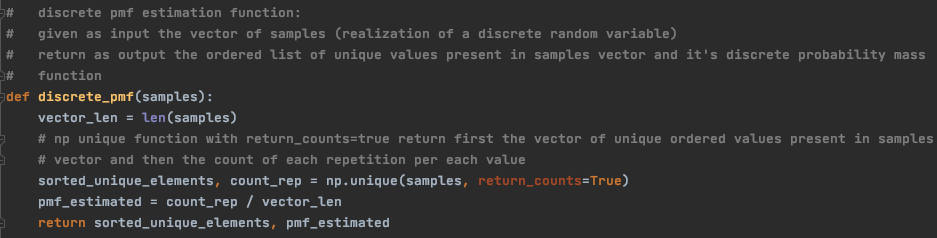
\includegraphics[width=16cm]{Pictures/pmf estimation.png}
    \caption{Pmf estimation function}
\end{figure}

\newpage
Now we can compute the entropy of this estimate pmf and then perform the difference between H1 and H2, the result is $H2(X) = 1.8601326339214919 $ and $ |H1(X) - H2(X)| = 0.013693289250476193$, then graphically the difference between estimated pmf and a priori pmf is the follow.

\begin{figure}[h!]
    \centering
    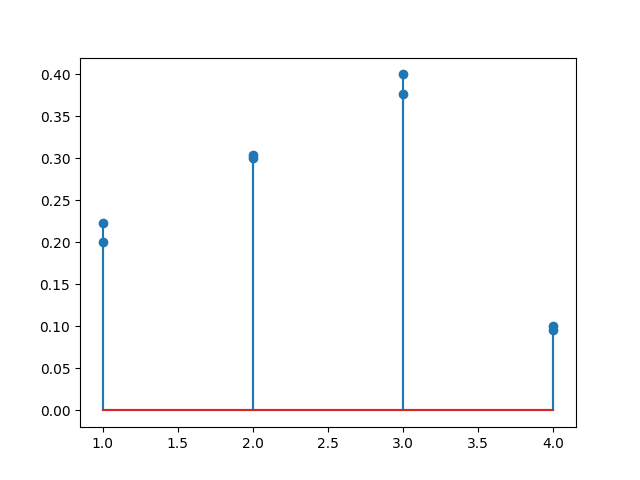
\includegraphics[width=13cm]{Pictures/p1-p2.png}
    \caption{Pmf estimated - pmf a priori}
\end{figure}

\section{Differential entropy}
In the case of continuous random variables we can define the differential entropy $h(X)$ computed given its
probability density function $f_{X}(X)$.
The difference with discrete case is that differential entropy is a relative measure of uncertain while in the 
discrete case is an absolute measure, in fact the domain of differential entropy can be any real number between 
$[-\infty,+\infty]$. Furthermore, the sum of the discrete case is replaced by the integral. In python the integral is solved by using quad method from library scipy.integrate as follow.

\begin{figure}[h!]
    \centering
    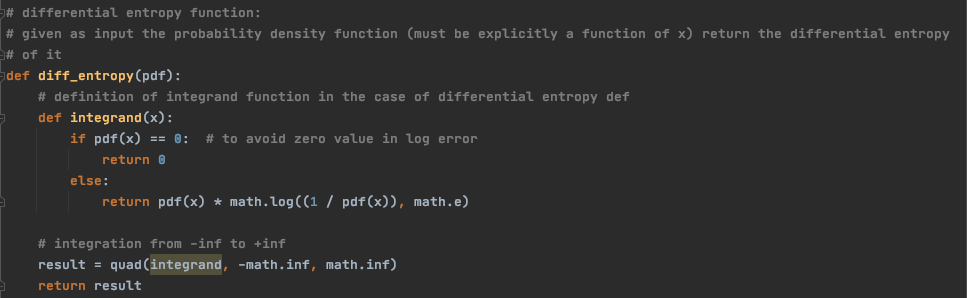
\includegraphics[width=15cm]{Pictures/Differential entropy fun.png}
    \caption{Differential entropy function}
\end{figure}

It's important to note that function accept in input an explicit function of x. To see if the function correctly work we can implement a uniform random variable density with parameter $a = 1/4$ and $b = 1/2$ as follow.

\begin{figure}[h!]
    \centering
    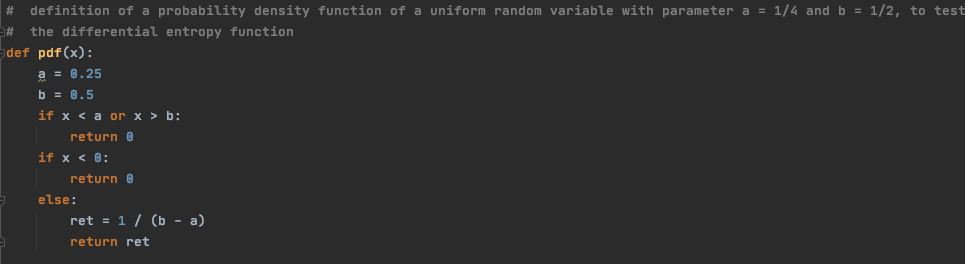
\includegraphics[width=15cm]{Pictures/Uniform pdf.png}
    \caption{Uniform pdf}
\end{figure}

Then by calling the differential entropy function and passing them the pdf of that uniform distribution we achieve the value $h(X) = -1.3862943611106981$ and if we use solve manually that integral we achieve $h(X) = ln(b-a) $ and it'possibile to verify that result is correct.

\section{Pdf estimator}
Now the request is to perform the same exercise of the pmf estimation (section 3.1), in this case for a continuous random variable and consequent for its probability density function. Given a continuous Gaussian random variable and its prior pdf we can calculate differential entropy. Then by creating a set of samples with the same pdf its possible to estimate the pdf and to compute the differential entropy of it. At the end is possible to see the difference between the two differential entropy. We can choose $mean = 5$ and $variance = 3$ for the Gaussian r.v. and then define the Gaussian pdf function as follow.

\begin{figure}[h!]
    \centering
    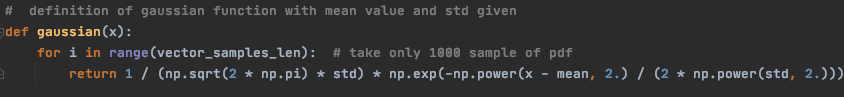
\includegraphics[width=15cm]{Pictures/Gaussian pdf.png}
    \caption{Gaussian pdf}
\end{figure}

Now we can simply compute the differential entropy by calling the precedent function and by passing the Gaussian fun. as parameter, we obtain $h1(X) = 2.5175508218727822$ for the differential entropy value. Now in 
order to estimate the Gaussian pdf we can first generate a set of 1000 samples normal distributed with random.normal() method of numpy library. Then it's possible to use kernel density estimation to compute the pdf 
suitable for these samples. But is also possible to use others method like the Histogram one. It is preferable to use the kernel method because even if we try to estimate a continuous function with Hystogram
we obtain a step function and inevitably it implies a loss of information. The kernel density estimator is smoother and converges as samples increase to the true probability density function. In order to apply it to 
generated samples, it is necessary to first estimate the variance and mean value of the samples. (Samples are generated with known pdf, but the estimate that is made is non-parametric, it is therefore assumed that the distribution of these samples is not known). Also in this case the choice of the bandwidth and the number of samples used greatly influences the final result of the estimation, choosing a too large band you risks underestimating the probability density in the densest areas. Choosing a too small  bandwidth you risks the overfitting (the model fits the data incorrectly). Consequently the choice that is made for an optimal band is the one made by experience and is the following shown in the next figure, furthermore to implement the kernel estimator it is possible to use the KernelDensity method from the sklearn.neighbors library.

\begin{figure}[h!]
    \centering
    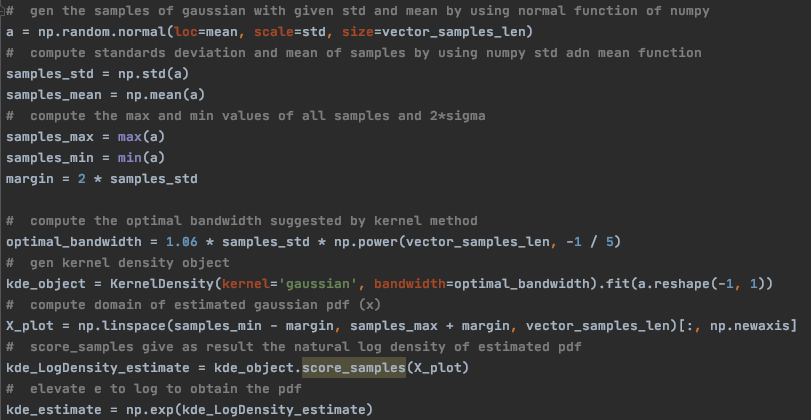
\includegraphics[width=16cm]{Pictures/pdf kernel estimator.png}
    \caption{Kernel density estimator}
\end{figure}

Considering that now the result of estimation is a vector of values fitted on a computed x domain to compute the differential entropy the precedent functions fail, because it work with explicit function of x and not with a vector. 
It is possible to solve this problem by using the simps function of scipy, passing to it a vector of values and the domain on which they are fitted returns the integral as a result. This solution is shown in the next figure.

\begin{figure}[h!]
    \centering
    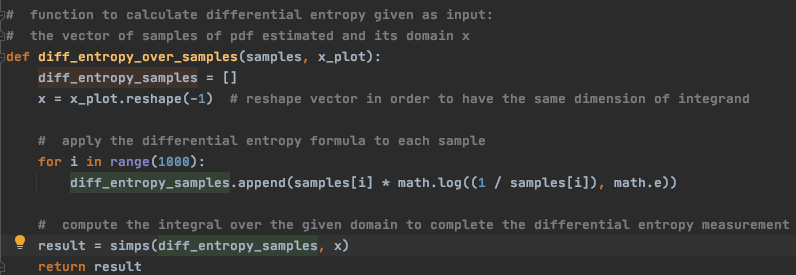
\includegraphics[width=15cm]{Pictures/Simps scipy.png}
    \caption{Diff. entropy with simps}
\end{figure}

\newpage
Now it's possibile to compute differential entropy of estimated pdf function and then compute
the difference with differential entropy of given prior pdf of the same data, the result is 
$h2(X) = 2.561244380941153$ and 
the difference is $|h1(x) - h2(x)| = 0.04369356$. If we use a optimal bandwidth and tophat kernel function the result is 
better $|h1(x) - h2(x)| = 0.01671652$.



\chapter{Assignment 4}

\section{Pmf Iris dataset}
The first requirements is to compute the probability mass function of the features of the Iris dataset after having discretized it as integers. First of all it is necessary to import the datasets method from the sklearns library through
which is possible to load the Iris dataset into a 150x4 matrix and its class vector. It is important to remember that the dataset class vector classifies each row of the dataset and assigns it to a specific class. In order to discretize the features is 
possible to iterate the dataset array for each row through a for loop, multiply the value of 
each instance by a constant (in this case 10) and cast the data to integer using the astype() method. Then we can pass each column discretized to the probability mass function estimator and save the result in a dictionary as shown in the next 
figure.

\begin{figure}[h!]
    \centering
    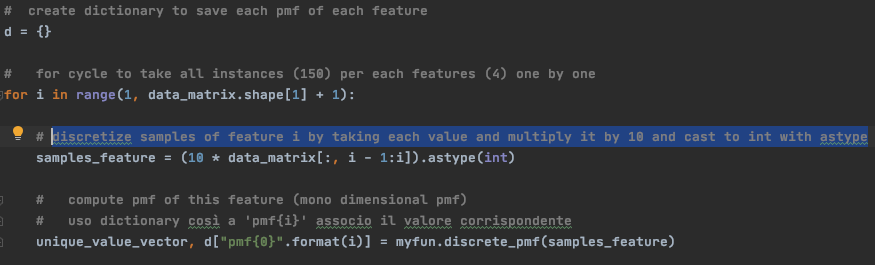
\includegraphics[width=15cm]{Pictures/Discretized iris.png}
    \caption{Pmf of iris dataset}
\end{figure}

the result is a dictionary containing the pmf vectors of the 4 features of the dataset and we can observe the dimensions and verify that the sum of each pmf is always unitary.

\begin{figure}[h!]
    \centering
    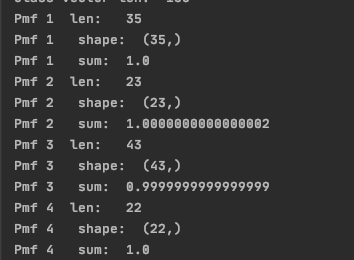
\includegraphics[width=10cm]{Pictures/Pmfs iris.png}
    \caption{Pmf of iris dataset}
\end{figure}



\section{Entropy}
The second request is to compute the entropy associated to each feature, it is perfomed by applying the discrete entropy function shown in the previous chapter to the pmf vectors just calculated, the result obtained is the following.

\begin{figure}[h!]
    \centering
    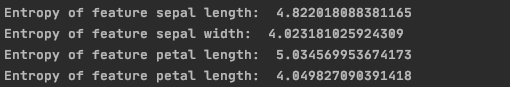
\includegraphics[width=10cm]{Pictures/Entropy iris.png}
    \caption{Entropy of iris dataset}
\end{figure}

\section{Mutual information}
The last request is to compute the mutual information between any pair of feature. In order to calculate the mutual information between any pair of features it is necessary to know the joint probability mass of the features in question and the marginal probabilities. So first you need to select the target features and discretize them as done previously. We select the first two features multiply them by 10 and cast them to integers. It is now possible to estimate the joint probability by extending the previous function pmf estimator univariate to the multivariate case as follow.

\begin{figure}[h!]
    \centering
    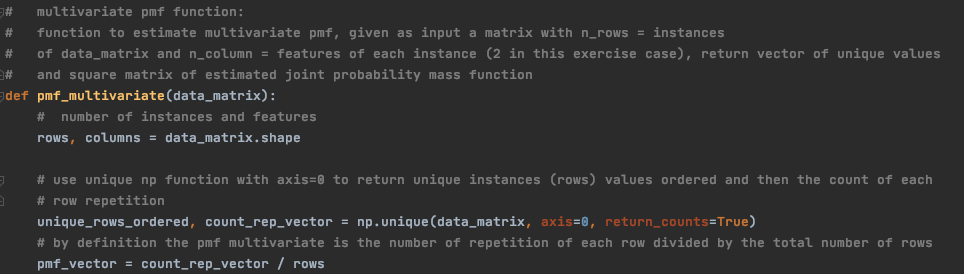
\includegraphics[width=15cm]{Pictures/Pmf multivariate estimator.png}
    \caption{Multivariate pmf estiamtor}
\end{figure}


Now to make the joint probability mass just estimated compatible with the mutual information function shown in the previous chapters, it is necessary to construct a square matrix in which to insert the data of the prob mass that are in form of a vector. We select the max and min value for each column and then compute the difference in order to select the max difference of values, it will be the dimension of square matrix in wich we will put the data. Next initialize a zeros matrix of that dimension and start to fill with pmf multivariate values. The value i of the vector pmf is inserted in position [uniquerows[i] - [xmin, ymin]]. A square matrix representative the joint probability mass function is achieved in this way. The process is shown in the next figure.

\begin{figure}[h!]
    \centering
    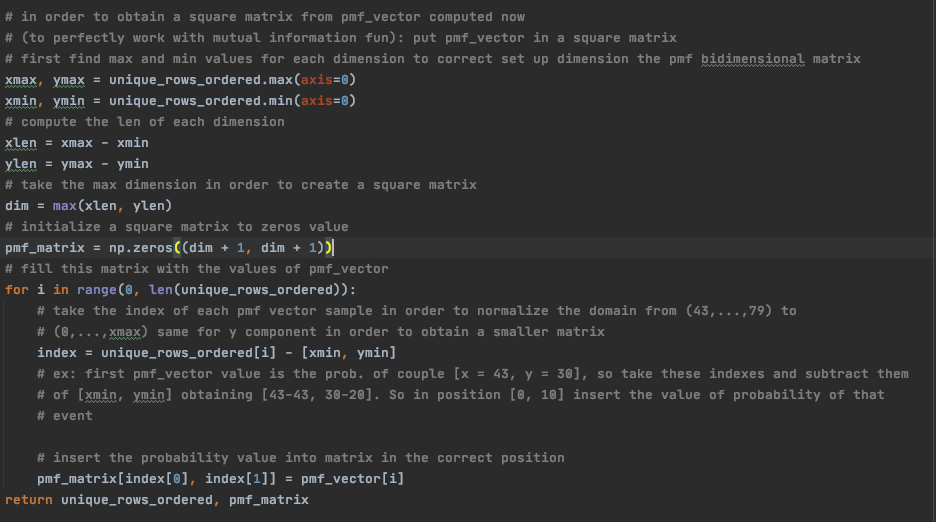
\includegraphics[width=16cm]{Pictures/Square matrix for pmf.png}
    \caption{Square matrix for pmf creation}
\end{figure}
\newpage
Now it's possible to apply the mutual information function shown in the precedent chapter to obtain the 
the result $I(X;Y) =  2.089844090533955$ also by applying the relationship between marginal entropy and
joint entropy the same result is achieved $I(X;Y) = H(X) + X(Y) - H(X,Y) =  2.089844090533955$. 
The obtained value demonstrate that the first two features of Iris dataset are nearly independent, because the max value that mutual information can assume in case of discrete r.v. is $min{H(X),H(Y)}$ and we can observe that $H(X)$ and $H(Y)$ are almost the double of the obtained value.



\chapter{Assignment 5}
\section{Bayes classifier}
The first request is to build a full bayes classifier which take in input the training dataset, the class vector of the training dataset and the test dataset, it will provide in output the class vector for the test dataset under the assumption that features are realizations of continuous random variables. So to correct estimate their pdf is needed to use the kernel density estimator. Recalling that the classification process is the learning from the training dataset of the relation $\hat{c} = f(x) $ that permit to predict the class label for a given instance. In particular in the Bayes classifier this mapping procedure is performed using Bayes' theorem. The goal of the classifier is to select the class $c_{j}$ for the instance under consideration such that it maximizes the posterior probability $P(c_{j}|x)$ which can be expressed through Bayes' theorem as follows 
$P(c_{j}|x) = P(x|c_{j}) P(c_{j})/ P(x)$. In order to maximize this value the denominator can be excluded from the calculations as it is always constant for every j.
Computed this value for the row under test and for each $c_{j}$ where $j$ goes from 0 to the total number of classes, then is selected the class label $c_{i}$ that maximize $P(c_{i}|x)$ and consequently the instance is linked to the relative class $i$.
This process permits to associate any instances to the class that most likely gave rise to the instance (likelihood concept).
Given the training dataset and the relative class vector, we can summarize the classification process as follow:

\begin{itemize}
\item training phase 1:
    \begin{itemize}
        \item estimation of the pmf of the training class label vector
    \end{itemize} \newpage
\item training phase 2:
    \begin{itemize}
        \item splitting the training dataset into N (len of class vector) sub datasets and estimate its probability density function of each part, this pdf estimated correspond to the conditional probability $p(x|c_{j})$
    \end{itemize}
\item test phase:
    \begin{itemize}
        \item  computing the class vector for the test dataset by test each row and assign them to class value which maximize posterior prob $p(c_{j}|x)$ expressed through the Bayes formula.
    \end{itemize}
\end{itemize}

The training phase 1 for estimating the pmf of class label vector is solved using the pmf estimator seen in the previous chapters.
The training phase 2 is solved by using a for cycle iterated over the length of the class vector, in order to divide the training dataset into equally size parts by calculating the length of each part as the total length of training dataset divided by the number of classes. Then for each sub dataset pdf is computed.

\begin{figure}[h!]
    \centering
    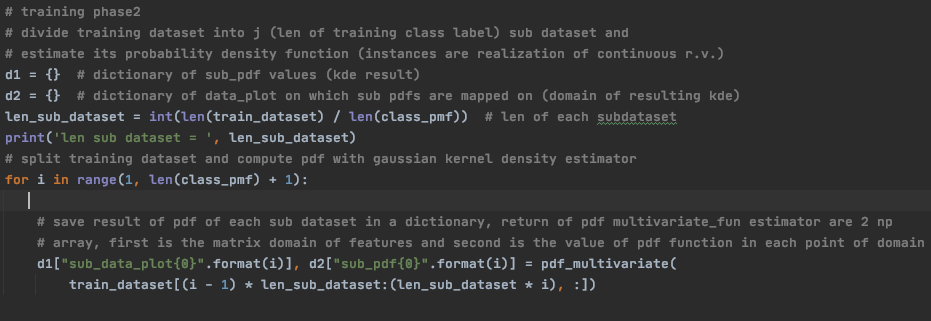
\includegraphics[width=15cm]{Pictures/training phase 2.png}
    \caption{Training phase 2}
\end{figure}

\newpage
We assume that features are realizations of continuous random variable so for each sub dataset the multivariate probability density function is estimated using the kernel function shown below. The pdf of each subset is saved by means of 2 dictionaries, in the first is saved the vector of kde values for each pdf and in the second is saved the domain on which it is fitted. Considering that we have 4 features we compute mean, std and domain for each 4.

\begin{figure}[h!]
    \centering
    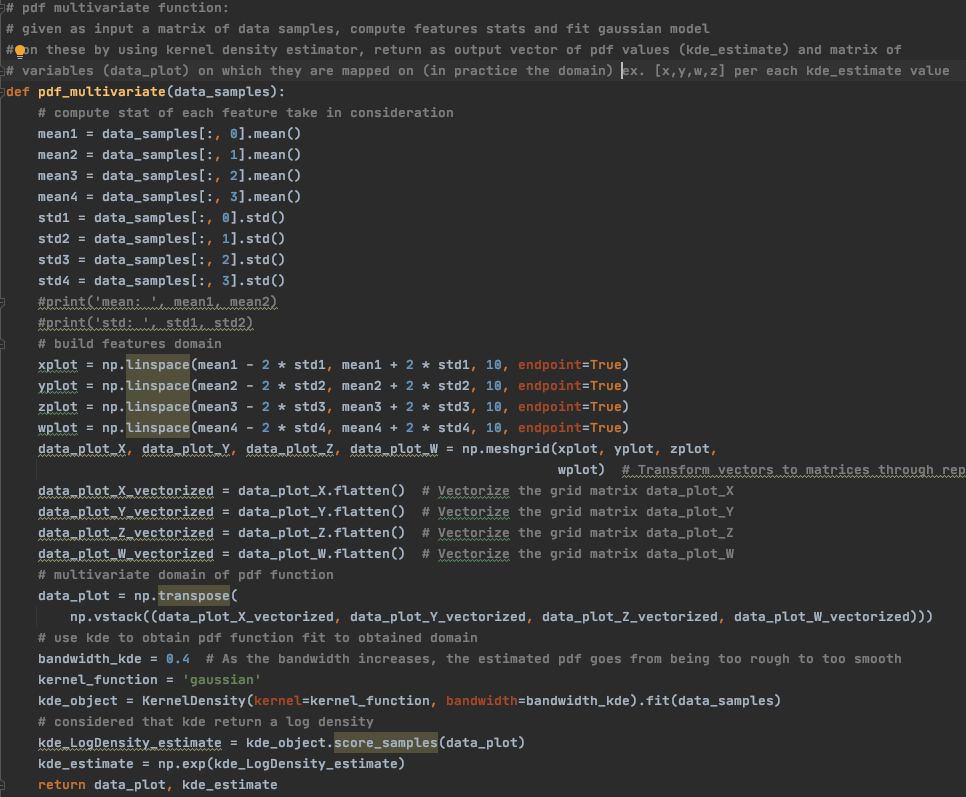
\includegraphics[width=15cm]{Pictures/pdf multivariate.png}
    \caption{Multivariate pdf}
\end{figure}

\newpage
Then the last phase is the test phase, we have multiavariate pdf for each sub dataset that in practice is the conditional probability in the Bayes formula. We have also the pmf of class vector and so we can compute the posterior probability through the Bayes theorem. So for each row (instances) of test dataset we can compute the conditional probability for each pmf value and class vector multiply them by pmf of $c_{j}$ in consideration and then select the max as follow.

\begin{figure}[h!]
    \centering
    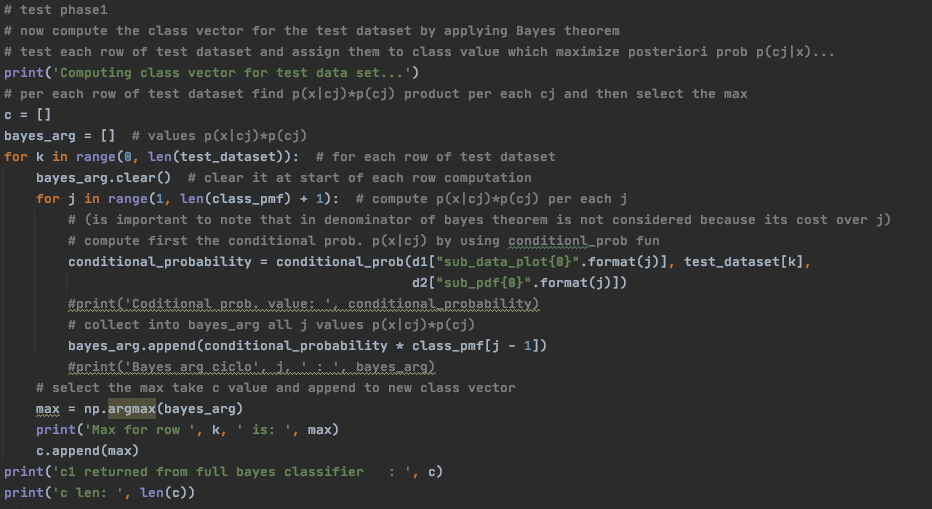
\includegraphics[width=16cm]{Pictures/test phase.png}
    \caption{Test phase}
\end{figure}

Then we collect for the same row of instances under test all the n (number of class) Bayes argument values and select the max among them. The $c_{j}$ selected is saved in the new class label vector.

\newpage
As we can see to compute the conditional probability we use a function that accept in input the kde estimated values, the domain on which they are fitted on and the test dataset instances. The work of this function is done as follow, first the 4 features of row under test are searched within the domain of the pdf (in data plot), the index of the domain vector whose values satisfy the almost equal match (because values are float) is taken and the value of the pdf is calculated at that point.

\begin{figure}[h!]
    \centering
    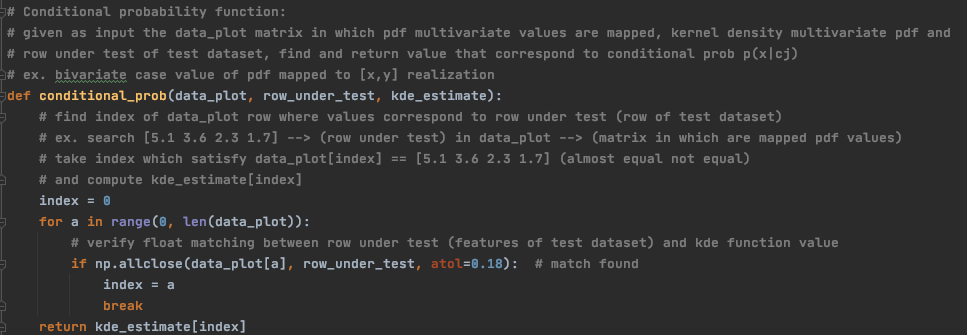
\includegraphics[width=16cm]{Pictures/Conditional prob.png}
    \caption{Conditional probability}
\end{figure}


In the end result of Bayes classifier function is a vector c class label suitable for the test data set.

\section{Naive Bayes classifier}

In order to build the naive Bayes classifier we can apply only small modification to the last function considering that in this condition each feature is independent from each others, so to compute the probability density function is possible to estimate first the marginal pdf of each feature and then by multiplying them we obtain the multivariate pdf. Each phase, traing phase 1, training phase 2 and test phase remain the same as previous, we can change only the function that compute the pdf and the conditional probabilities as follow.

\begin{figure}[h!]
    \centering
    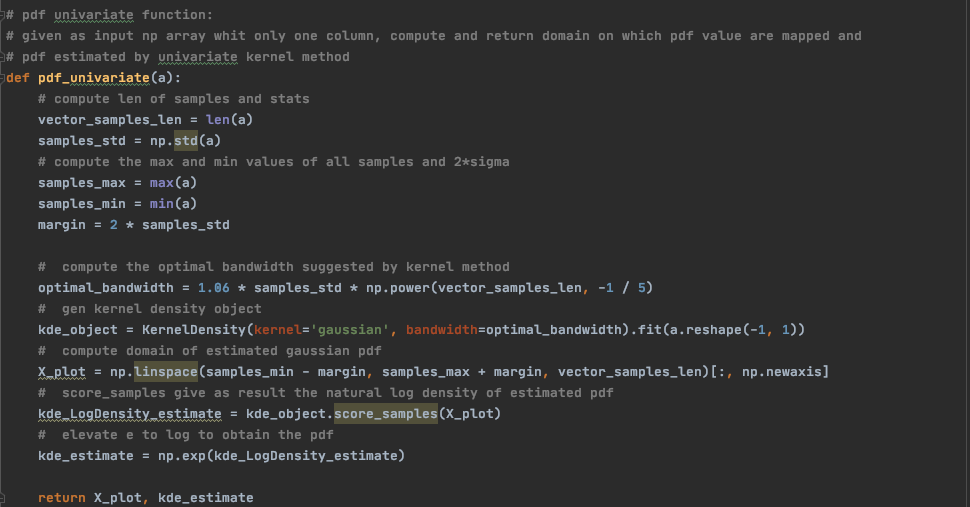
\includegraphics[width=16cm]{Pictures/Univariate pdf.png}
    \caption{Univariate pdf estimation}
\end{figure}

\newpage
We perform this computation per each feature so at the end we have 4 marginal pdf saved into 4 dictionaries because for each pdf we again have two elements: the domain and the values of the fitted function on it. Then during the test phase we compute the conditional probabilities by using new function at which we pass all the marginal pdfs. As previous for each pdf it's necessary to retrieve the domain index for which the almost equal condition between instance under test and point domain is satisfied. At the end the function return the product of each computed pdf value as follow. There are 4 for loops like the next picture shows that make up the function, each for the 4 feature. In input the function need also the j index, number of class vector that is under testing.


\begin{figure}[h!]
    \centering
    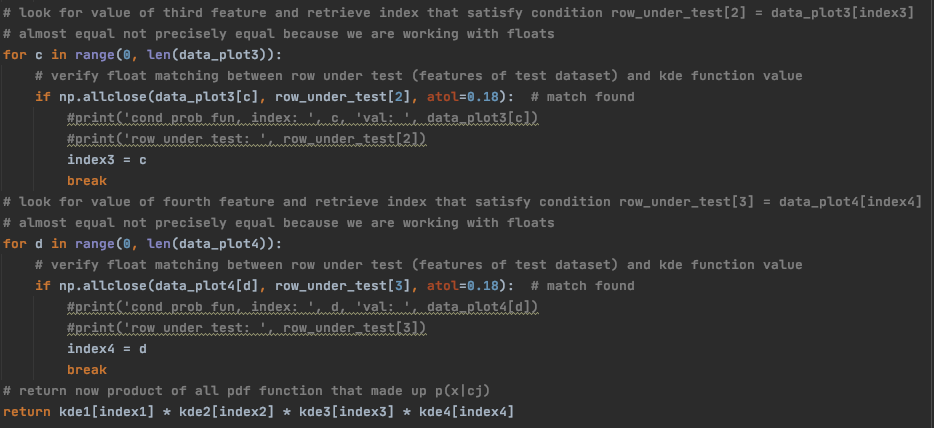
\includegraphics[width=16cm]{Pictures/Naive conditional prob.png}
    \caption{Naive conditional probability}
\end{figure}

\newpage
Then the last test phase computations remain the same as previous.
\section{Naive Bayes classifier with parametric estimation}
The third request is to build a Naive Bayes classifier under the assumption that each features is the realization of continuous random variables as precedent request but it is now assumed that the distribution is Gaussian. Under these hypotheses it is now possible to make a parametric estimation of the probability densities unlike before that a non-parametric estimation was made. Therefore, to derive the probability density of each feature it is possible to directly use the formula of the Gaussian distribution. The only parameters to be estimated remain the mean and the standard deviation. So the training phase 1 remain always the same, we can estimate the pmf of training class vector by using the pmf estimator function as usual. Then during the training phase 2, as usual we can split the training dataset in 4 sub dataset (eah for class) and in order to estimate the marginal pdf of each feature now we can simply estimate the mean and std. As we can see in the next picture the   training phase 2 is done by splitting the training dataset as usual and then by simply computing the mean and std for each feature and for each class.


\begin{figure}[h!]
    \centering
    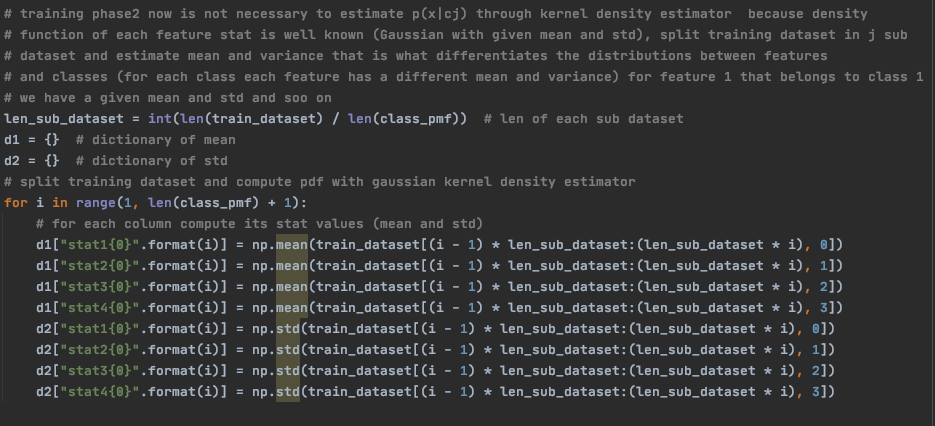
\includegraphics[width=13cm]{Pictures/Training phase naive gaussian.png}
    \caption{Naive Gaussian training phase}
\end{figure}

Then during the test phase in order to compute the Bayes argument and retrieve the maximum value, for each row (instances) we can compute the conditional probabilities $p(x|c_{j})$ by use the univariate Guassian equation with given mean and std as follow.

\begin{figure}[h!]
    \centering
    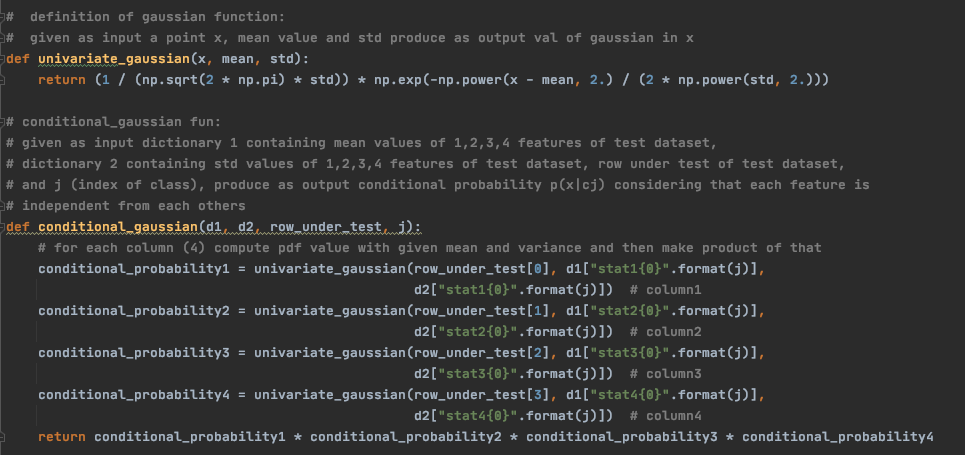
\includegraphics[width=16cm]{Pictures/Test phase naive gaussian.png}
    \caption{Naive Gaussian test phase}
\end{figure}
\newpage
\section{Accuracy comparison}
Now having the three different versions of the Bayes calassifier available, we can test their accuracy using them on the Iris dataset. In particular, by examining 50\% of each class as a training dataset and the remaining 50\% as a test dataset, using the 3 different classifiers the following results are obtained.

\begin{figure}[h!]
    \centering
    
\includegraphics[width=16cm]{Pictures/Final accuracy.png}
    \caption{Accuracy of classifiers}
\end{figure}

To perform these accuracy measurements it's possible to use the method metrics from the library sklearn, by calling metric.accuracy-score() and by passing them the computed class vector and the real one it return the accuracy of measurements. If we use a kernel other than the Gaussian one in pdf kernel estimation we achieve lower accuracy result as shown in the next figures.

\begin{figure}[h!]
    \centering
    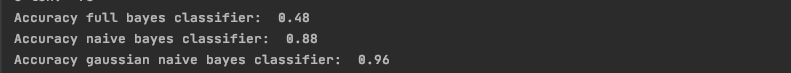
\includegraphics[width=14cm]{Pictures/epanechnikov kernel accuracy.png}
    \caption{Accuracy with Epanechnikov kernel function}
\end{figure}

\begin{figure}[h!]
    \centering
    
\includegraphics[width=14cm]{Pictures/tophat kernel accuracy.png}
    \caption{Accuracy with Tophat kernel function}
\end{figure}

The best result is achieved using the Gaussian kernel function with bandwidth equal to 0.5.

\begin{figure}[h!]
    \centering
    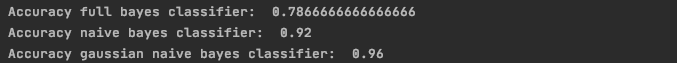
\includegraphics[width=14cm]{Pictures/best accuracy.png}
    \caption{Accuracy with Gaussian kernel function and 0.5 bandwidth}
\end{figure}


\end{document}
